\documentclass[12pt]{article}
\usepackage{amsmath, amsfonts, dsfont}
\usepackage{enumitem}
\usepackage{graphicx}
\usepackage[margin=1in]{geometry}
\usepackage{hyperref}
\usepackage{siunitx}
%\usepackage[nomarkers]{endfloat}
\PassOptionsToPackage{hyphens}{url}
\hypersetup{linktoc=all}
\usepackage[style=authoryear,maxcitenames=2,backend=biber]{biblatex}
\addbibresource{refs.bib}
% chktex-file 24
% chktex-file 27

\title{Addicted to Dropping Out: \\ Opioids and Labor Force Participation\thanks{I thank Simon J\"ager for his guidance and help throughout this project and in writing this paper.}}
\author{Oscar Suen\thanks{Massachusetts Institute of Technology, \href{mailto:osuen@mit.edu}{\texttt{osuen@mit.edu}}}}
\date{\today}

\begin{document}
\maketitle

\begin{abstract}
\noindent Using the differential impact of the introduction of Medicare Part D as an instrument for opioid supply, we measure the causal impact of the opioid epidemic on labor force participation and other labor market outcomes.  We find that an increase of 1 standard deviation in the long-difference of opioids per capita in a commuting zone leads to a $1.4$ percentage point decrease in the labor force participation rate.  
% TODO: reframe numbers
There is no significant effect on incomes for the employed, but there is an increase in the percentage of people earning zero income.  Moreover, effects are stronger for men than for women, and are concentrated among those aged 25--44.  Finally, an event study suggests that effects take time to materialize.
\end{abstract}

\newpage
\section{Introduction} \label{introduction}
Over the last two decades in the US, two parallel trends stand out: the massive increase in opioid use and the secular decline in the labor force participation rate.  Prescription opioid abuse led the way to a full-blown opioid epidemic, which killed on average 130 people a day in 2017.~\footfullcite{epidemic} Simultaneously, the prime age labor force participation rate reversed a decades-long rise, falling from $84.0\%$ in 2000 to $81.6\%$ in 2011,~\footfullcite{fred-lfp} bringing potential challenges for the US economy.

With these trends occurring over the same time period, the question is whether they are linked in some way, and specifically whether the worsening opioid epidemic caused adverse labor market outcomes.  Figure~\ref{figure:opioidandlfp} shows the parallel trends, and illustrates the stunning increase in the amount of opioids prescribed in the US, which more than quadrupled from 2000 to 2011.  We can imagine that this correlation actually stems from some causal pathway.  For workers without steady employment, opioid use might push them out of the labor force if their drug addiction affects their work.  \textcite{miamidrugs} present evidence that substance abuse in general has negative effects on employment, with chronic drug use having a marginal effect of $-10\%$ on the probability of employment.  There may be spillover effects as well.  Family members of addicts may drop out of the labor force to care for their relatives.  Businesses may also decide to lower wages in or even move out of areas where the epidemic is widespread.  \textcite{mullahy93} and \textcite{kaestner94} give evidence that alcoholism and illegal drug use respectively have a negative impact on wages.  All of these potential mechanisms could be part of a causal relationship between opioid use and labor market outcomes.  

\begin{figure}[htbp]
    \centering
    \caption{Opioids per Capita and Prime Age Labor Force Participation in the US}
    \begin{minipage}{0.8\textwidth}
    \includegraphics[width=\textwidth]{figs/graph_opioidlfp.pdf}
    \footnotesize
    The blue line with the left axis shows the morphine-equivalent grams of opioids prescribed per person in America from 2000--2016.  For context, a standard Vicodin pill has $7.5$ morphine-equivalent milligrams.  The red line with the right axis shows the prime-age (25--54) labor force participation rate over the same period.
    \end{minipage}
    \label{figure:opioidandlfp}
\end{figure}

\textcite{krueger17} shows that there is a cross-county correlation between opioid prescriptions in 2015 and the drop in labor force participation from 2000 to 2015.  Extrapolating from the regression coefficient, the increase in opioid prescriptions over 1999--2015 accounted for a 0.6\% drop in the male labor force participation rate, which is about 20\% of the total drop.  This provides some additional quantitative evidence for a relationship between the opioid epidemic and depressed labor force participation.

However, there is still an identification challenge in trying to estimate the causal effect instead of just the correlation.  \citeauthor{krueger17}'s results do not rule out an omitted variable causing both an increase in opioid abuse and adverse labor market outcomes nor a causal pathway in reverse.  Worsening labor market conditions could drive people to abuse opioids when they are laid off.  \textcite{hollingsworth17} suggest that a 1\% increase in the unemployment rate is associated with a $3.6\%$ increase in overdose deaths.  However, \textcite{ruhm18} suggests that there is no relationship between the economic conditions in a county and the overdose death rate after accounting for selection.  In any case, there are serious concerns about endogeneity in studying this relationship.
% TODO: Look at Cleveland Fed paper

In this paper, we study the causal impact of opioids on the labor market.  We look at the effect of opioid prescriptions per capita on labor market outcomes in a commuting zone.  We instrument opioid use with the differential impact of Medicare Part D across commuting zones.  The introduction of Medicare Part D provided a plausibly exogenous increase in opioid prescriptions in a commuting zone, which allows us tease out the causal effect on local labor markets.

The opioid epidemic in the US has garnered much media attention over the last few years, and for good reason.  The Center for Disease Control estimates that 11.5 million people misused prescription opioids in 2016.~\footfullcite{hhs-about}  This drug epidemic is different from others in US history in that drug users often start with legal prescription medication.  A variety of opioids are commonly prescribed as painkillers, including hydrocodone (Vicodin) and oxycodone (Percocet and Oxycontin).  Anecdotal evidence suggests that in recent years many of those addicted to prescription painkillers move on to illegal opioids like heroin and fentanyl.  This in total caused 116 deaths a day in 2016 from opioid-related overdoses.  Figure~\ref{figure:opioidandlfp} shows just how fast the increase in prescriptions has been over the last two decades.  For reference, the standard Vicodin pill has $7.5$ morphine-equivalent milligrams, which means that in 2011, the equivalent of $72$ Vicodin pills were being prescribed for every man, woman, and child in America.  While these massive numbers can be partially explained by the availability of opioids in massive doses (such as the $120$ morphine-equivalent milligram Oxycontin pill), they still illustrate the enormity of the amount of opioids prescribed in the US\@.

In 2003, Congress passed Medicare Part D, a program subsidizing the costs of prescription drugs for those on Medicare, which provides government insurance for seniors aged 65 and over.  In 2017, 42 million people received subsidies for prescription drugs through the program,~\footfullcite{kff-partd} showing its widespread adoption.  The program started in 2006, and generally lowered the cost of prescription drugs for the elderly.  Presumably, making prescription opioids cheaper for the elderly increases the total amount of opioids prescribed.  Since the elderly share in areas around the country are significantly different, the program had a differential impact geographically.  

Our empirical strategy works because Medicare Part D as a policy choice is plausibly exogenous to local labor market conditions.  Since we are looking at prime age labor force participation, which only includes those aged 25--54, direct effects from the introduction of Medicare Part D are potentially less relevant.  The instrument captures an exogenous increase in the opioid supply in an area.  We suggest that the robust secondary market in opioids then allows for prime-aged workers to have access to opioids prescribed to the elderly.  \textcite{schnell17} gives evidence that the secondary market for opioids is large enough that it influences prescribing decisions.  There is also ample anecdotal evidence that the secondary market is an important mechanism in the worsening epidemic.  Purdue Pharma, which manufactures Oxycontin, was revealed to have had knowledge of the exact price of its drug ``on the street''.~\footfullcite{purduescandal}  The \emph{Charleston Gazette-Mail} reported that a single pharmacy in West Virginia purchased $10.9$ million doses of hydrocodone from 2007--12 in a shocking example of the ``pill mill'' phenomenon.~\footfullcite{charlestongazette}  In a particularly brazen scheme, two Alabama doctors opened up a clinic with an adjacent pharmacy that once sold more than $\$570\,000$ worth of an extremely potent opioid nominally used only for terminal cancer patients in a single month.  The parking lot outside pharmacy reportedly always had a few people camped out trying to buy opioids.~\footfullcite{painhustlers}  In Dreamland,~\footfullcite{dreamland} \citeauthor{dreamland} writes that ``Some of the first Oxy[contin] dealers\ \dots\ were seniors who saw the value of the pills in their cabinet''.  All of this suggests that the secondary market is an important component of the opioid crisis, and that increased availability of opioids to the elderly increased availability to the prime-aged population as well.

Once people get addicted to opioids through the increased supply, the epidemic can also cascade.  Friends of addicts could take up opioids as well, and those who were only mildly addicted could see their addictions worsen.  This suggests that the exogenous shock from the instrument should have increasing effects over time.

The causal mechanism that we suggest follows a paper by \textcite{alpert17}.  They exploit a similar differential impact of Medicare Part D as an instrument for consumer drug advertising to study the effect on drug utilization.  We also follow \textcite{powell15}, who study the first stage effects of Medicare Part D on state-level opioid prescriptions.  We expand this analysis to the commuting zone level to obtain more precise estimates which more accurately captures effects on individual communities.  We then exploit this relationship to study causal impacts of the opioid crisis on the labor market.

The remainder of the paper is laid out as follows.  Section~\ref{estimation} discusses in detail our estimation strategy.  Section~\ref{data} discusses the sources for our data and presents summary statistics for variables of interest.  Section~\ref{results} presents results.  Finally, Section~\ref{conclusion} concludes.

\section{Estimation Strategy} \label{estimation}
\subsection{Difference-in-Difference Instrument}
The proposed empirical test is to exploit the differential geographic impact of the introduction of Medicare Part D as an instrument for the supply of prescription opioids to study the impact on labor market outcomes.  Prescriptions of opioids to the elderly are a significant portion of overall opioid prescriptions, 
% TODO: do we want to find data on this?
and Medicare Part D made prescriptions much cheaper to obtain for the elderly, so we should expect there to be a strong first stage.  Our instrument is also plausibly exogenous to labor market conditions.  For exogeneity to be violated, we would need there to be some reason, other than the differential impact of Medicare Part D on the opioid supply, that CZs with a higher elderly share affected the labor market but only after 2006.  The fact that Medicare Part D provided benefits for the elderly while we look at effects on the prime-aged labor market lends credibility to this assumption.

Our strategy is related to the one employed by \textcite{powell15}.  We expand their analysis by using the commuting zone level instead of the state level, giving a more fine-grained look at the data.  We do this mainly because the mechanism described is more likely to occur at the local level, and running the analysis on the state level might not capture it.  The secondary market for opioids is often a decentralized network of drug dealers or even individuals selling their prescription opioids to friends.~\footfullcite{dreamland}  These street sales are likely to occur within local labor markets, which are more accurately described by commuting zones than by states.  The more detailed geography also allows division-by-year fixed effects to control for differential time trends in different parts of the country.

Specifically, the first-stage regression is
\[ \mathit{Prescriptions}_{tc} = \beta(\mathit{\%65plus}_{2003,c}\cdot\mathds{1}_{t\geq2006}) + \alpha_{d(c)t} + \gamma_c + \varepsilon_{tc} \]
where $t$ is the year (possibility of using quarterly data too), $c$ is the commuting zone (or zip code).  $\mathit{Prescriptions}$ is the morphine-equivalent weight of opioids prescribed, which varies by commuting zone and year.  $\mathit{\%65plus}$ is the share of population who are aged 65 or over, which here is fixed at the proportion in 2003 when Medicare Part D was announced.  We fix the year at 2003 to remove any potential endogeneity arising from migration from the announcement of the policy.  The coefficient of interest is then on the interaction between the introduction of Medicare Part D and the number of old people, which gives an index of how much Medicare Part D affected a county.  We then add census division $\times$ year fixed effects $\alpha_{d(c)t}$ where $d(c)$ is the census division containing the commuting zone $c$, and commuting zone fixed effects $\gamma_c$.

We then look at the effect of opioid prescriptions with:
\[ Y_{tc} = \theta\mathit{Prescriptions}_{tc} + \tau_{d(c)t}+ \sigma_c + \eta_{tc} \]
where $Y$ is a labor market outcome, and $\mathit{Prescirptions}$ is instrumented as above.  We will primarily focus on the labor force participation rate, but we also look at unemployment, income, and share with zero income in a commuting zone.  We then disaggregate these labor market outcomes by age, gender, and race to look at the effect on population subgroups.

We use a two-stage least squares IV estimator to get an estimate of how opioid prescriptions affect the labor market.

The IV estimation strategy laid out solves a few problems that a direct OLS would have.  An OLS estimate is biased by potential reverse causality.  If labor market conditions affect the opioid prescription rate, which is supported by evidence by \textcite{hollingsworth17}, then when we estimate the OLS coefficient, there is reverse causality bias to make the OLS estimate unreliable.  The instrument overcomes this by using a plausibly exogenous source of variation in the opioid prescription rate.  If the exclusion restriction holds (discussed below), then the instrument measures what happens after opioids are exogenously introduced in an area, which allows us to obtain causal estimates of the effect of the opioid crisis on the labor market.

The regressions also include division-by-year and CZ fixed effects.  These fixed effects should take out any possible omitted variables that would bias the estimates.  CZ fixed effects controls for demographic and other fixed characteristics by local area.  The division-by-year fixed effects allows for each census division to have a different non-linear time trend, which takes out the effect of prescriptions increasing yearly over the period of interest.

\subsection{Event Study}
Since labor markets may take time to adjust to an increase in opioids, we also want to look at an event study.  More specifically, we look at the coefficients of the first stage and reduced form equations:
\begin{align*}
    \mathit{Prescriptions}_{tc} &= \sum_{k=2000}^{2011}\beta_k(\mathit{\%65plus}_{2003,c}\cdot\mathds{1}_{t=k}) + \alpha_{d(c)t} + \gamma_c + \varepsilon_{tc} \\
    Y_{tc} &= \sum_{k=2000}^{2011} \theta_k(\mathit{\%65plus}_{2003,c}\cdot\mathds{1}_{t=k}) + \tau_{dt} + \sigma_c + \eta_{tc}
\end{align*}
The event study allows us to see the effect of the increase in opioids due to Medicare Part D over time.  The coefficients $\theta_k$ then show the effect of the shock over time.  The framework also allows us to examine any pretrend as a falsification test.  If the elderly share in a CZ has an effect before the introduction of Medicare Part D (i.e.\ before 2006), there may be a violation of the exclusion restriction.

% TODO: maybe discuss long difference regression

\subsection{Assumptions}
The key identification strength comes from the fact that the instrument acts primarily on the elderly population, while we look mainly at labor market outcomes among the working aged.  This of course does not remove all possible exogeneity concerns, but is a good first approximation.  We are thus relying on the fact that the sole causal channel works through the increased availability of opioids on the secondary market caused by cheaper prescription drugs to the elderly from Medicare Part D.
% TODO: look at this sentence again.

The main assumption for a difference-in-difference design is parallel trends.  Here, this corresponds to the assumption that in the scenario without Medicare Part D, the number of opioid prescriptions in commuting zones with a large elderly proportion would have changed in the same way as the number in CZs with a small elderly proportion.
% TODO: this sounds wrong, maybe conditional on fixed effects?

To test this assumption, we can look at the pretrends in the event study.  Specifically, we can see how the instrument affects opioid supply from 2000--2005.  An effect of zero would tend to support the assumption that trends in opioid supply would have been similar without the 2006 introduction of Medicare Part D.  It is also important to note that if there is a slight linear pretrend in the first stage regression but not the reduced form regression, the identification still holds, because if the first stage is biased away from zero, the IV coefficient is biased towards zero.
% TODO: recheck that the years line up (survey year vs.\ when part D started)

The assumptions for instrumental variables estimation are a strong first stage and the exclusion restriction.  We can test for a strong first stage with the first stage regression.  The exclusion restriction remains an assumption though.  Specifically here, we require that the differential impact of Medicare Part D in 2006 from different elderly populations only affects the labor market through the mechanism of increasing the supply of opioids.  This is not an unreasonable assumption, since we are looking at two separate groups (the labor market consists of people under 65).  
% However, there could potentially be problems associated with migration, where young people move out of stagnant labor markets and old people do not, creating an increase in the share of the elderly. 
% TODO: commented out sentence sounds untrue.

\section{Data} \label{data}
\subsection{Data Sources}
We use microdata from the Census Bureau hosted on IPUMS-USA.~\footfullcite{ipums}  Specifically, we use the 2000 decennial Census for data in 2000 and the yearly American Community Survey (ACS) from 2005--11.  The Census and the ACS both have individuals as their unit.  This allows direct calculation of means in each geographic area.
% TODO: robustness check using 1990 census?

Geographic information for every observation is only available for the Census and the ACS after 2005, which is why the period of analysis does not cover 2001--04.  Specifically, the Census Bureau codes Public Use Microdata Areas, which are geographic areas large enough to report.  The way we generate means for different geographic levels is described in the section on Geographic Divisions.

The Census and ACS include labor market outcomes and demographic information.  Labor force participation is defined as employment status being employed or unemployed.  Unemployment is defined as unemployed if participating in the labor force.  We use the raw annual income measure to construct log real income deflated to 2000 USD with the Core CPI deflator (Consumer Price Index for All Urban Consumer: All Items Less Food and Energy).~\footfullcite{fred-cpi}

We then use demographic information to construct mean labor market outcomes in each commuting zone for prime-aged (25--54) workers.  We then further break down the population into subgroups by age and sex.
% TODO: are there any limitations to the IPUMS data?

To measure the spread of the opioid epidemic, we use data from the ARCOS~\footfullcite{arcos} system maintained by the DEA, which has data from 2000--16.  The DEA mandates that pharmacies report the total amounts of controlled substances prescribed.  It then reports the total weight of each type of drug prescribed in each 3-digit ZIP code prefix every quarter in an annual report.

The ARCOS data gives a very precise and accurate look at the number of opioid prescriptions, but it may not track the intensity of the opioid epidemic in an area exactly.  There are two possible misalignments.  Firstly, most descriptions of the opioid epidemic include illegal drugs like heroin and fentanyl, which we do not capture here.  Secondly, we observe the ZIP code of prescription instead of the location of consumption.  While our use of commuting zones aims to capture the local area of economic activity, and so it is plausible that most opioid prescribed in a commuting zone are also consumed in the same commuting zone, we cannot account for the possibility that certain pharmacies (the so called ``pill mills'') supply a much larger area of opioid consumption.
% TODO: maybe include measures of state laws in covariates?

In light of these limitations of the data, our results should be interpreted as the causal impact of more opioid prescriptions in an area instead of the causal impact of the opioid epidemic.  However, anecdotally, many addicts who abuse illegal drugs like heroin and fentanyl started off with prescription opioids, so the epidemic is inextricably and tightly linked with prescription opioids.
% TODO: try to find better evidence and cite
In addition, policymakers may be more interested in controlling the supply of prescription opioids than the considerably harder task of restricting the consumption of illegal drugs.  Our analysis then presents the total causal impact of an increase in opioid prescriptions, which includes the impact of addicts who transition from prescription opioids to illegal opioids, on the labor market.

We use the data from ARCOS on prescriptions for various forms of opioids by 3-digit ZIP code prefix.  We convert each type of opioid into its equivalent morphine weight using the Morphine Milligram Equivalent (MME) conversion table~\footfullcite{mme} to standardize the measure.  The list of opioid compounds measured and the MME conversion rates are presented in Table~\ref{table:opioidmme}.  The totals are summed to get a measure of the total amount of opioids prescribed yearly, and then divided by population to get the per capita prescription rate.  Again, the method for changing geographic aggregation levels is described in the Commuting Zone section.

To get a sense of the units used here, a single Percocet contains around 5 MMEs, while a pill of Oxycodone has 15 MMEs.  Prescriptions for wisdom teeth are around 12 pills for a total of around 50 MMEs.  Formulations for patients with very high tolerance can have up to 100 MMEs in a single pill, but 100 MMEs also carries a much higher risk of overdose for patients with normal tolerance levels \parencite{nihoverdose}.
% TODO: maybe move this, this is the third time

\begin{table}
    \footnotesize
    \centering
    \caption{Opioids and Morphine Equivalents}
    \begin{tabular}{r|l}
\hline\hline
Opioid Drug & mg Morphine \\
\hline
Dihydrocodeine & 0.25\\
Hydrocodone & 1 \\
Hydromorphone & 4 \\
Levorphanol & 11 \\
Meperidine & 0.1 \\
Morphine & 1 \\
Oxycodone & 1.5 \\
\hline\hline
\end{tabular}

    \label{table:opioidmme}
\end{table}

\subsection{Geographic Divisions}
Our geographic unit of analysis for local labor markets is the 2000 Commuting Zone (CZ).  Commuting zones are clusters of counties that cover the US such that labor market activity is mostly confined within the CZ\@.  We use the 2000 version of commuting zones since our analysis mainly occurs in the 2000s.  There are 709 CZs, which gives enough power for analysis while maintaining a reasonable level of geographic aggregation.  The crosswalk file linking counties to CZs is from the Department of Agriculture Economic Research Service.~\footfullcite{czones}

The problem with commuting zones is that neither the Census data nor the ARCOS data reports by that geographic area.  So we have to impute values to each CZ based on allocation factors.  We use crosswalk files from MABLE~\footfullcite{geocorr} that link 5-digit ZIP codes and PUMAs to counties with population weights.  Following \textcite{dorn09}, we calculate \[ \alpha_{pz} = \sum_{c\in C(z)}\frac{\mathit{pop}_{pc}}{\mathit{pop}_c} \] where $\alpha_{pz}$ is the allocation factor for PUMA $p$ to CZ $z$, $\mathit{pop}_{pc}$ is the population in both PUMA $p$ and county $c$, $\mathit{pop}_c$ is the population in county $c$, and $C(z)$ is the set of counties in CZ $z$.  Populations are based on Census estimates in 2000.

We have to do something a little more complicated with 3-digit ZIP code prefixes, but similarly, we have \[ \alpha_{tz}=\sum_{c\in C(z)}\sum_{f\in F(t)}\frac{\mathit{pop}_f}{\mathit{pop}_t}\frac{\mathit{pop}_{fc}}{\mathit{pop}_f} \] where $t$ is a 3-digit ZIP code prefix, $f$ is a 5-digit ZIP code, $c$ is a county, $z$ is a commuting zone, $C(z)$ is the set of counties in CZ $z$, and $F(t)$ is the set of 5-digit ZIP codes with 3-digit prefix $t$.

To get the CZ level variables for, say, number of prescriptions, which are measured for every 3-digit ZIP code prefix, we just impute using the allocation factors,
\[ \mathit{Prescriptions}_{z} = \sum_{t} \alpha_{tz} \mathit{Prescriptions}_{t} \]
Most of the $\alpha_{tz}$s will be 0, except for the 3-digit zip code prefixes $t$ which intersect the commuting zone $z$.  Other variables on the CZ level are constructed similarly.

We can think about both allocation factors in terms of probability.  In the first case, it is fairly simple.  We allocate a person according to the population probability to a commuting zone.  In the second case, we have to assume some notion of independence, but we essentially allocate a prescription in a 3-digit ZIP prefix to one of its 5-digit ZIP codes, then across into a county, and then a CZ\@.

To measure the elderly share in each commuting zone, we use population data from the Census Population Estimates~\footfullcite{censuspop}, which includes data on population by county for each age group.  We use the share of population that is aged 65 or over as a proxy for the utilization of Medicare (and hence the impact of the introduction of Medicare Part D) in each geographic area.  We also use total population counts to weight geographic areas.

\subsection{Descriptive Statistics}
The data used is a balanced panel of year and Commuting Zones.  The panel includes the years 2000 and 2005--11.  There are 709 consistent CZs in each year, which gives a total of $N=5672$.  The summary statistics in tables below, when weighted, are weighted by the population share in each commuting zone in 2003.

\subsubsection{Instrument}
The instrument used is based on the elderly share (share of population aged over 65) in each commuting zone in 2003.  The weighted mean of the variable is $0.146$ and the standard deviation is $0.296$.  
% TODO: Weighted SD doesn't make sense??
% TODO: Add 25-75th percentiles for context?
To see the distribution of the instrument among commuting zones, a histogram of values is presented as Figure~\ref{figure:sholdhist}.  This shows that the instrument has significant variation and is distributed normally, both of which give confidence in the instrument's power.  Finally, we present at a map of the elderly shares in each commuting zone in Figure~\ref{figure:sholdmap}.  While there is some clustering geographically, there is also significant variation within states.

\begin{figure}[htbp]
    \centering
    \caption{Histogram of Elderly Share in 2003 by CZ}
    \begin{minipage}{0.8\textwidth}
    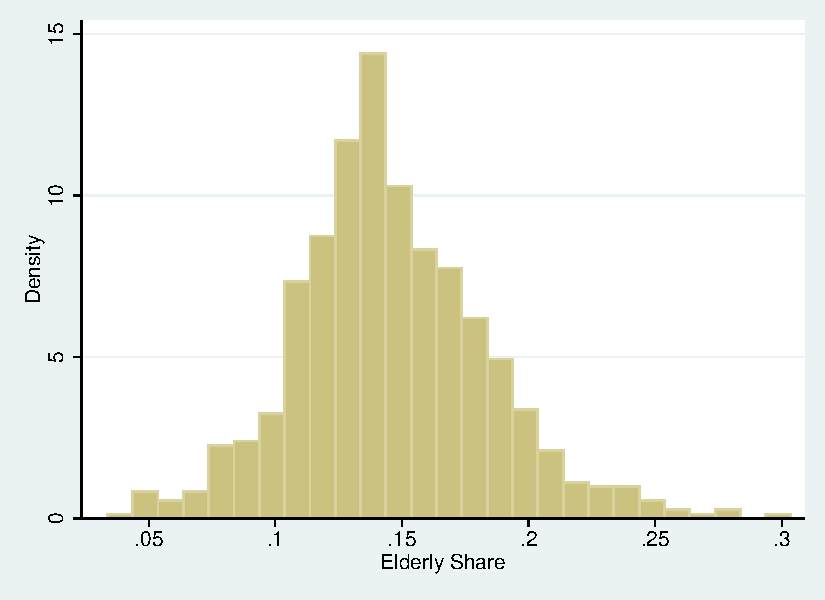
\includegraphics[width=\textwidth]{figs/hist_shold.pdf}
    \footnotesize
    Unweighted histogram of elderly share by CZ in 2003. $N=709$.
    \end{minipage}
    \label{figure:sholdhist}
\end{figure}

\begin{figure}[htbp]
    \centering
    \caption{Map of Elderly Share in 2003 by CZ}
    \begin{minipage}{\textwidth}
    \includegraphics[width=\textwidth]{figs/map_shold.pdf}
    \footnotesize
    Map by CZ of elderly share in 2003 for each CZ\@.  Darker areas have higher elderly share.
    \end{minipage}
    \label{figure:sholdmap}
\end{figure}

\subsubsection{Opioid Prescriptions}
A weighted summary table for opioid prescriptions per capita in morphine equivalent grams by commuting zone is presented as Table~\ref{table:opioidsumm}.  The first row is the aggregate of all observations over all years.  The mean increases almost linearly over the years.  The standard deviation also seems to increase more than the mean, suggesting a divergence between commuting zones over time.

\begin{table}
    \footnotesize
    \centering
    \caption{Summary of Opioid Prescription Rates}
    {
\def\sym#1{\ifmmode^{#1}\else\(^{#1}\)\fi}
\begin{tabular}{l*{1}{cccc}}
\hline\hline
            &        Mean&          SD&         Min&         Max\\
\hline
Overall Opioid Prescriptions&       0.401&       0.182&       0.064&       1.227\\
Opioid Prescriptions (2000)&       0.131&       0.058&       0.022&       0.497\\
Opioid Prescriptions (2001)&       0.198&       0.081&       0.033&       0.528\\
Opioid Prescriptions (2002)&       0.226&       0.092&       0.038&       0.598\\
Opioid Prescriptions (2003)&       0.267&       0.108&       0.040&       0.730\\
Opioid Prescriptions (2004)&       0.291&       0.121&       0.040&       0.843\\
Opioid Prescriptions (2005)&       0.305&       0.127&       0.043&       0.892\\
Opioid Prescriptions (2006)&       0.357&       0.153&       0.049&       1.061\\
Opioid Prescriptions (2007)&       0.422&       0.193&       0.069&       1.250\\
Opioid Prescriptions (2008)&       0.442&       0.202&       0.083&       1.372\\
Opioid Prescriptions (2009)&       0.485&       0.243&       0.077&       1.703\\
Opioid Prescriptions (2010)&       0.526&       0.285&       0.074&       2.149\\
Opioid Prescriptions (2011)&       0.537&       0.245&       0.085&       1.651\\
$\Delta$ Opioid Prescriptions (2000--2011)&       0.406&       0.204&       0.063&       1.491\\
$\Delta$ Opioid Prescriptions (2000--2005)&       0.174&       0.085&       0.021&       0.608\\
$\Delta$ Opioid Prescriptions (2006--2011)&       0.179&       0.119&      -0.075&       0.985\\
\hline
\(N\)       &         709&            &            &            \\
\hline\hline
\multicolumn{5}{p{0.65\textwidth}}{Summary of opioid prescriptions per capita in morphine equivalent grams at the CZ level.  Weighted by population in 2003.  Long difference calculated by CZ.}
\end{tabular}
}

    \label{table:opioidsumm}
\end{table}

We can see the change in opioid prescriptions over time in Figure~\ref{figure:opioidandlfp}, which shows the total amount of opioids prescribed in the US over 2000--16 in millions of morphine equivalent grams.  The number more than triples over the period of analysis, showing the rapid escalation of the epidemic.  There appears to be an inflection around 2006, which would support our empirical strategy of using the increase in opioids from the expansion of Medicare Part D.
% TODO: don't know if talking about this inflection is good

Lastly, we present a map of CZs (Figure~\ref{figure:opioidmap}) colored by the long difference in per capita prescriptions.  Here we see significant geographic heterogeneity.  The map shows the severity of the opioid epidemic in Appalachia and Ohio, which are commonly cited as the worst-hit areas of the epidemic.  However, New England does not show up as a hard-hit area, possibly because the epidemic in New England has been driven mostly by heroin and fentanyl.  We also see hotspots in the Northwest and in Florida, which are less commonly associated with the epidemic.

\begin{figure}[htbp]
    \centering
    \caption{Map of the Long Difference (2000--2011) in Opioid Prescription Rates by CZ}
    \begin{minipage}{\textwidth}
        \includegraphics[width=\textwidth]{figs/map_opioiddiff.pdf}
    \footnotesize
    Map by CZ of long difference in opioid prescription rate (morphine-equivalent grams per capita).
    \end{minipage}
    \label{figure:opioidmap}
\end{figure}

\subsubsection{Labor Market Outcomes}
Weighted summary statistics for labor force outcomes are presented in Table~\ref{table:laborsumm}.  We present statistics for four variables here: labor force participation, unemployment, log real income, and percent with no income.  All statistics are weighted by CZ population in 2003.  Statistics are calculated as means of binary variables, except for log real income, which is calculated as a weighted median.  We examine three potential definitions of ``prime-aged.''  Using ages 16--64 uses the full sample excluding the elderly; using ages 16--54 strips out possible forward looking effects from older workers; using ages 25--64 tries to exclude the effect of schooling; and using the BLS specification of 25--54 strips out early retirement too.  Following the BLS, we will use ages 25--54 as our definition.  We also include statistics broken down by gender, as well as statistics for different age groups.

\begin{table}
    \scriptsize
    \centering
    \caption{Summary Table for Labor Market Statistics}
    {
\def\sym#1{\ifmmode^{#1}\else\(^{#1}\)\fi}
\begin{tabular}{l*{1}{cccc}}
\hline\hline
            &        Mean&          SD&         Min&         Max\\
\hline\hline
\multicolumn{5}{l}{Labor Force Part.}\\
\hline\hline
16--64     &       0.709&      0.0412&       0.473&       0.847\\
16--54     &       0.728&      0.0405&       0.502&       0.873\\
25--64     &       0.756&      0.0422&       0.494&       0.891\\
25--54     &       0.797&       0.039&       0.549&       0.919\\
\hline
16--24     &       0.578&      0.0573&       0.296&       0.773\\
25--34     &       0.803&      0.0417&       0.452&       0.945\\
35--44     &       0.803&      0.0379&       0.533&       0.959\\
45--54     &       0.788&      0.0448&       0.484&       0.942\\
55--64     &       0.606&      0.0627&       0.267&       0.823\\
\hline
25--54 Male  &       0.864&      0.0409&       0.485&       0.962\\
25--54 Female  &        0.74&      0.0465&       0.481&       0.908\\
\hline\hline
\multicolumn{5}{l}{Unemployment}\\
\hline\hline
16--64   &      0.0926&      0.0306&      0.0182&       0.298\\
16--54   &      0.0988&      0.0325&      0.0175&       0.322\\
25--64   &      0.0692&      0.0271&      0.0124&        0.25\\
25--54   &      0.0725&      0.0284&      0.0088&       0.274\\
\hline
16--24   &       0.178&      0.0508&      0.0233&       0.645\\
25--34   &      0.0898&      0.0354&           0&       0.376\\
35--44   &      0.0681&       0.028&           0&       0.267\\
45--54   &      0.0607&      0.0267&           0&       0.231\\
55--64   &      0.0539&      0.0254&           0&       0.202\\
\hline
25--54 Male &      0.0777&      0.0332&     0.00501&       0.339\\
25--54 Female &      0.0673&      0.0259&           0&       0.241\\
\hline\hline
\multicolumn{5}{l}{Log Real Income}\\
\hline\hline
16--64 &        10.2&       0.216&        9.31&        10.8\\
16--54 &        10.2&       0.209&        9.26&        10.7\\
25--64 &        10.5&       0.218&        9.58&          11\\
25--54 &        10.5&       0.213&         9.6&          11\\
\hline
16--24 &        8.85&       0.223&         7.7&        9.96\\
25--34 &        10.3&       0.202&        9.39&        10.8\\
35--44 &        10.6&       0.233&        9.65&        11.1\\
45--54 &        10.6&       0.221&        9.62&        11.2\\
55--64 &        10.5&       0.245&        9.47&        11.2\\
\hline
25--54 Male &        10.6&       0.207&        9.68&        11.1\\
25--54 Female &        10.3&       0.229&        9.44&        10.9\\
\hline\hline
\multicolumn{5}{l}{\% w/ No Income}\\
\hline\hline
16--64 &       0.297&      0.0516&       0.159&       0.565\\
16--54 &       0.276&       0.053&       0.136&       0.566\\
25--64 &        0.27&      0.0438&       0.154&       0.526\\
25--54 &       0.231&       0.041&       0.121&       0.509\\
\hline
16--24 &       0.373&      0.0852&      0.0787&       0.759\\
25--34 &       0.206&      0.0449&      0.0711&       0.548\\
35--44 &        0.23&      0.0402&      0.0974&       0.533\\
45--54 &       0.255&      0.0465&       0.128&        0.52\\
55--64 &       0.413&      0.0562&       0.223&       0.727\\
\hline
25--54 Male &       0.183&      0.0462&      0.0688&       0.579\\
25--54 Female &       0.272&      0.0472&       0.119&       0.494\\
\hline\hline
\(N\)       &        5672&            &            &            \\
\hline\hline
\multicolumn{5}{p{0.4\textwidth}}{LFP, Unemployment, No Income are percentages by CZ\@.  Log Real Income is adjusted by CPI (see text) and is the median by CZ\@.  Statistics reported over 2000 and 2005--2011 (the sample).  Weighted by population in 2003.}
\end{tabular}
}

    \label{table:laborsumm}
\end{table}

Our main variable of interest is prime age labor force participation.  We shows some additional descriptives about this variable in a map (Figure~\ref{figure:lfpmap}).  We map the long difference between 2000 and 2011 of LFP with areas with a bigger decline in LFP in a darker color.  There is considerable heterogeneity in LFP decline, both between states and within states.
% TODO: how is long difference related to diff-in-diff?

\begin{figure}[htbp]
    \centering
    \caption{Map of Long Difference (2000--2011) in Labor Force Participation by CZ}
    \begin{minipage}{\textwidth}
    \includegraphics[width=\textwidth]{figs/map_lfpdiff.pdf}
    \footnotesize
    Map of long difference (2000--2011) in prime age (25--54) labor force participation rate by CZ\@.
    \end{minipage}
    \label{figure:lfpmap}
\end{figure}
% TODO: make time period of long difference consistent
% TODO: census vs ACS problem in map?

\section{Results} \label{results}
\subsection{First Stage}
We first look at the relationship between the difference-in-difference instrument and opioid prescription.  The first stage results are shown in Table~\ref{table:firststage}.  Here we are regressing opioid prescription rates on the Medicare Part D impact instrument (Elderly Share in 2003 $\times$ Post-2006).  The first column shows our preferred specification, which includes Census division $\times$ year fixed effects, CZ fixed effects, and is weighted by population in 2003.  We also present coefficients from the other possible specifications.  Column 2 shows the simple unweighted bivariate regression of the two variables.  Column 3 include only year and CZ fixed effects.  Column 4 is an unweighted version of our preferred specification.  Column 5 includes state-by-year fixed effects instead of by division.  Finally column 6 includes a linear time-trend (Elderly Share $\times$ Year).  In all specifications, standard errors are clustered by commuting zone.

\begin{table}
    \footnotesize
    \centering
    \caption{First Stage: Effect of Instrument on Opioid Prescription Rate}
    {
\def\sym#1{\ifmmode^{#1}\else\(^{#1}\)\fi}
\begin{tabular}{l*{6}{c}}
\hline\hline
            &\multicolumn{1}{c}{(1)}        &\multicolumn{1}{c}{(2)}        &\multicolumn{1}{c}{(3)}        &\multicolumn{1}{c}{(4)}        &\multicolumn{1}{c}{(5)}        &\multicolumn{1}{c}{(6)}        \\
\hline
Instrument  &        2.25\sym{**}&        1.22\sym{**}&        2.18\sym{**}&        0.72\sym{**}&        1.05\sym{**}&        0.45\sym{**}\\
            &      (0.41)        &     (0.059)        &      (0.46)        &      (0.12)        &      (0.23)        &      (0.14)        \\
[1em]
\hline
Year FE     &          Div        &          No        &         Year        &          Div        &          State        &          Div        \\
CZ FE       &          Yes        &       No             &          Yes        &          Yes        &          Yes        &          Yes        \\
Weighted    &     Yes        &           No         &     Yes        &       No             &     Yes        &     Yes        \\
Time Trend    &     No        &           No         &     No        &       No             &     No        &     Yes        \\
\hline
$\bar{R}^2$ &        0.78        &        0.15        &        0.72        &        0.78        &        0.87        &        0.79        \\
$N$         &        5672        &        5672        &        5672        &        5672        &        5672        &        5672        \\
\hline\hline
\multicolumn{7}{p{0.6\linewidth}}{\footnotesize Standard errors in parentheses.  First stage OLS estimates for opioid prescription rate presented.  Instrument is elderly share in 2003 $\times$ post-2006.  Year FE row denotes whether the specification included no year FEs, year FEs, division $\times$ year FEs, or state $\times$ year FEs.  CZ FE row denotes whether specification included commuting zone fixed effects.  Weighting (when used) by population in 2003 and equal across years.  Time trend is elderly share in 2003 $\times$ year.  Standard errors clustered by CZ. \sym{*} \(p<0.05\), \sym{**} \(p<0.01\)}\\
\end{tabular}
}

    \label{table:firststage}
\end{table}

We use the specification in column 1 as our preferred specification.  We would like to include census division $\times$ year fixed effects to take out different time trends by each geographic area, and we would like to weight our counties to get a sense of the average impact over the US\@.

Our preferred specification is highly statistically significant, with an $F$-statistic of $30$, which is significant enough to use as a first stage regression in the TSLS regressions that follow.  
% TODO: Get more precise F-stat
We also show a bin-scatter plot in Figure~\ref{figure:binscatter} of the first stage, showing a tight relationship between our instrument and our regressor.  We have also included two alternative specifications as robustness checks.  Column 5, which allows for differential state time trends, shows that our results still hold even if we restrict the variation to within states.  Column 6 shows that adding a time trend reduces the point estimate, but the coefficient is still significant.  We discuss this more in the event study analysis.

\begin{figure}[htbp]
    \centering
    \caption{Bin-Scatter Plot for First Stage Regression}
    \begin{minipage}{0.8\textwidth}
    \includegraphics[width=\textwidth]{figs/graph_binscatter.pdf}
    \footnotesize
    Bin-scatter plot of the first stage relationship between the instrument and the opioid prescription rate.  Includes division-by-year and CZ FEs. Weighted by population in 2003.
    \end{minipage}
    \label{figure:binscatter}
\end{figure}

The magnitude of the effects are significant.  The coefficient suggests that a $1$pp higher elderly share in a CZ is associated with an increase of $22.5$ MMEs of opioids prescribed per person after Medicare Part D in 2006.  The mean of the prescription rate in 2006 was $0.36$, which corresponds to an effect of around $6\%$.  While this comparison is not a direct causal effect, this also corresponds to around $5\%$ of the change in prescriptions per person over 2000--2011.
% TODO: interpretation of moving from 10--90th percentile
% TODO: 1 SD in elderly share is $3.8$pp

\subsection{Second Stage}
Table~\ref{table:tsls} shows the results for the OLS (1), reduced form (2), and TSLS (3) regressions for the main variables of interest for prime age workers.  All specifications include division-by-year and CZ fixed effects, are weighted by population in 2003 and equally by year, and standard errors are clustered by CZ\@.

\begin{table}
    \footnotesize
    \centering
    \caption{OLS, Reduced Form, and TSLS Estimation}
    {
\def\sym#1{\ifmmode^{#1}\else\(^{#1}\)\fi}
\begin{tabular}{l*{3}{c}}
\hline\hline
            &\multicolumn{1}{c}{(1)}&\multicolumn{1}{c}{(2)}&\multicolumn{1}{c}{(3)}\\
            &\multicolumn{1}{c}{OLS}&\multicolumn{1}{c}{Red.\ Form}&\multicolumn{1}{c}{TSLS}\\
\hline\hline
Labor Force Part.\\
\hline
Opioid Rate &     $-0.0093$        &                    &      $-0.069$\sym{**}\\
            &    (0.0087)        &                    &     (0.025)        \\
[1em]
Instrument  &                    &       $-0.16$\sym{**}&                    \\
            &                    &     (0.043)        &                    \\
\hline
$\bar{R}^2$ &        0.57        &        0.58        &        0.43        \\
\hline\hline
Unemployment \\
\hline
Opioid Rate &       0.022\sym{**}&                    &       0.034\sym{**}\\
            &    (0.0044)        &                    &     (0.012)        \\
[1em]
Instrument  &                    &       0.077\sym{**}&                    \\
            &                    &     (0.027)        &                    \\
\hline
$\bar{R}^2$ &        0.86        &        0.86        &        0.84        \\
\hline\hline
Log Real Income \\
\hline
Opioid Rate &      $-0.053$\sym{**}&                    &       0.023        \\
            &     (0.015)        &                    &     (0.046)        \\
[1em]
Instrument  &                    &       0.052        &                    \\
            &                    &      (0.10)        &                    \\
\hline
$\bar{R}^2$ &        0.96        &        0.96        &        0.95        \\
\hline\hline
\% w/ No Income\\
\hline
Opioid Rate &       0.016\sym{*} &                    &       0.027\sym{*} \\
            &    (0.0062)        &                    &     (0.014)        \\
[1em]
Instrument  &                    &       0.061\sym{*} &                    \\
            &                    &     (0.029)        &                    \\
\hline
$\bar{R}^2$ &        0.70        &        0.70        &        0.66        \\
$N$         &        5672        &        5672        &        5672        \\
\hline\hline
\multicolumn{4}{p{0.5\linewidth}}{\footnotesize Standard errors in parentheses.  All regressions include division-by-year and CZ fixed effects. Weighted by population.  Standard errors are clustered by CZ.  Outcomes for people aged 25--54.  \sym{*} \(p<0.05\), \sym{**} \(p<0.01\)}\\
\end{tabular}
}

    \label{table:tsls}
\end{table}
% TODO: What does this actually show??
% TODO: Want to include OLS coefficients

%%%%%%%%%%%%%%%%%%%% Editing Process %%%%%%%%%%%%%%%%%%%%

The OLS coefficients and the IV coefficients above show that endogeneity is a serious concern, which is not surprising given the potential for reverse causality, where a deteriorating labor market pushes affected workers to opioid abuse.  We show the OLS coefficients only for reference, and they should not be taken as meaningful numbers.  We discuss the significance and magnitudes of the IV results in the next section.

\subsection{Main Results}
Table~\ref{table:mainresults} show the TSLS panel regression coefficients for opioid prescription rates for four labor market outcomes and four specifications of ``prime-aged'' workers.  Each row in the table represents a different labor market outcome, and each column represents a different age range specification.  Again all regressions are weighted by population in 2003 and equally by year, and include division $\times$ year and CZ fixed effects.  Standard errors are clustered by CZ as usual.

\begin{table}
    \footnotesize
    \centering
    \caption{Effect of Opioid Crisis on Labor Market Outcomes}
    {
\def\sym#1{\ifmmode^{#1}\else\(^{#1}\)\fi}
\begin{tabular}{l*{4}{c}}
\hline\hline
            &\multicolumn{1}{c}{(1)}&\multicolumn{1}{c}{(2)}&\multicolumn{1}{c}{(3)}&\multicolumn{1}{c}{(4)}\\
            &\multicolumn{1}{c}{16--64}&\multicolumn{1}{c}{16--54}&\multicolumn{1}{c}{25--64}&\multicolumn{1}{c}{25--54}\\
\hline\hline
Labor Force Part.\\
\hline
Opioid Rate &      $-0.024$        &      $-0.038$\sym{*} &      $-0.050$\sym{*} &      $-0.069$\sym{**}\\
            &     (0.018)        &     (0.018)        &     (0.023)        &     (0.025)        \\
\hline
$\bar{R}^2$ &        0.40        &        0.38        &        0.45        &        0.43        \\
\hline\hline
Unemployment \\
\hline
Opioid Rate &       0.023        &       0.031\sym{*} &       0.025\sym{*} &       0.034\sym{**}\\
            &     (0.015)        &     (0.015)        &     (0.012)        &     (0.012)        \\
\hline
$\bar{R}^2$ &        0.84        &        0.84        &        0.85        &        0.84        \\
\hline\hline
Log Real Income \\
\hline
Opioid Rate &       0.084        &       0.062        &       0.029        &       0.023        \\
            &     (0.050)        &     (0.048)        &     (0.043)        &     (0.046)        \\
\hline
$\bar{R}^2$ &        0.94        &        0.92        &        0.96        &        0.95        \\
\hline\hline
\% w/ No Income \\
\hline
Opioid Rate &     $-0.0030$        &       0.012        &      0.0072        &       0.027\sym{*} \\
            &     (0.015)        &     (0.016)        &     (0.013)        &     (0.014)        \\
\hline
$\bar{R}^2$ &        0.81        &        0.82        &        0.68        &        0.66        \\
$N$         &        5672        &        5672        &        5672        &        5672        \\
\hline\hline
\multicolumn{5}{p{0.55\linewidth}}{\footnotesize Standard errors in parentheses.  Regressions include division-by-year and CZ FEs.  Weighted by population.  Standard errors clustered by CZ.  \sym{*} \(p<0.05\), \sym{**} \(p<0.01\)}\\
\end{tabular}
}

    \label{table:mainresults}
\end{table}
% TODO: use two-way clustering by CZ and year?

Some of these coefficients are statistically significant.  Across different age-range specifications, the effects all have the expected sign.  Our preferred specification seems to give the most power.  We restricted the definition to exclude effects on those close to retirement and young workers, as well as to conform with the standard definition of prime-aged workers.  Workers close to retirement could be affected more directly by the expansion of Medicare Part D, which would violate our exclusion restriction.  We show a further breakdown of results by age later.

The point estimates are very large.  An increase of 1 standard deviation in the long difference ($0.2$ grams) of opioids prescribed in a CZ causes a $1.38$ percentage point decrease in the prime age labor force participation rate.  By comparison, BLS data shows that the prime age LFP decreased by $2.4$pp from 2000--2011.~\footfullcite{fred-lfp}  While there is no clear way to directly compare these numbers, since our methodology looks at the cross-sectional variation instead of variation over time, our results do suggest that the opioid crisis contributed heavily to the drop in the prime age LFP rate.
% TODO: other ways to look at the magnitude (90--10? 75--25?)

We see similar significant effects on unemployment and percentage with no income.  A 1 standard deviation in the long difference of opioid prescribed per person causes a $0.68$pp increase in the unemployment rate and a $0.54$pp increase in the percentage of people with no income.  However, income does not seem to be affected.  The point estimate is an increase of $0.04$ log points per standard deviation increase in the long difference, and is not statistically significant.

Our results are consistent with a story where the opioid epidemic causes addicts to drop out of the labor force or get fired.  Employers may not directly lower wages in response to a crisis, especially if labor supply decreases.  This may also be because mostly low-wage workers are affected by our causal mechanism.  The average wage of the remaining workers would then increase, potentially offsetting any negative effects.

These results are similar to those found by \textcite{harris18}, who use the location of opioid ``pill mills'' as an instrument.  They however point in a different direction from \textcite{currie18}, who find a small positive effect of opioid prescriptions on employment-to-population ratios using opioid prescriptions for the elderly as an instrument.  We find our results more convincing because our instrument does not suffer from potential endogeneity concerns.  The location of ``pill mills'' is not exogenous and is probably driven by opioid demand.  The robust secondary market also suggests that opioid prescriptions may not ultimately be taken by the patient they are prescribed to, which would make prescriptions to the elderly endogenous to labor market conditions as well.
% TODO: add actual numbers
% TODO: cite new Cleveland Fed results

\subsection{Detailed Results}
% TODO: add race/education analysis
% TODO: effects by sector??
% TODO: effects on income terciles?
We present the regression results broken down by gender in Table~\ref{table:bysex}.  The coefficients for male labor force indicators are all larger than those for females.  For example, LFP drops by $2.4$pp for men versus $0.8$pp for women in response to a standard deviation increase in the long difference of opioid prescriptions.  The stunning magnitude of the point estimate for male LFP suggests that the opioid epidemic played a huge role in decreasing LFP among men.

\begin{table}
    \footnotesize
    \centering
    \caption{Effect of Opioid Crisis by Gender}
    {
\def\sym#1{\ifmmode^{#1}\else\(^{#1}\)\fi}
    \begin{tabular}{l*{2}{c}}
\hline\hline
            &\multicolumn{1}{c}{(1)}&\multicolumn{1}{c}{(2)}\\
            &\multicolumn{1}{c}{Male}&\multicolumn{1}{c}{Female}\\
\hline\hline
Labor Force Part.\\
\hline
Opioid Rate &       $-0.12$\sym{**}&      $-0.035$\sym{*} \\
            &     (0.038)        &     (0.018)        \\
\hline
$\bar{R}^2$ &        0.21        &        0.43        \\
\hline\hline
Unemployment \\
\hline
Opioid Rate &       0.042\sym{**}&       0.024        \\
            &     (0.012)        &     (0.013)        \\
\hline
$\bar{R}^2$ &        0.81        &        0.74        \\
\hline\hline
Log Real Income \\
\hline
Opioid Rate &      $-0.050$        &       0.071        \\
            &     (0.045)        &     (0.047)        \\
\hline
$\bar{R}^2$ &        0.93        &        0.94        \\
\hline\hline
\% w/ No Income \\
\hline
Opioid Rate &       0.057\sym{**}&      0.0012        \\
            &     (0.020)        &     (0.014)        \\
\hline
$\bar{R}^2$ &        0.65        &        0.42        \\
$N$         &        5672        &        5672        \\
\hline\hline
\multicolumn{3}{p{0.4\linewidth}}{\footnotesize Standard errors in parentheses.  Outcomes for ages 25--54.  Regressions include division-by-year and CZ FEs.  Weighted by population.  Standard errors clustered by CZ.  \sym{*} \(p<0.05\), \sym{**} \(p<0.01\)}\\
\end{tabular}
}

    \label{table:bysex}
\end{table}

The larger effect of the opioid crisis on men squares well with literature starting with \textcite{casedeaton}, who explored ``deaths of despair'' concentrated among men.  While the opioid epidemic is not solely a male phenomenon, the labor market effects seem to hit men much harder.  We can potentially interpret this in the framework of ``resilience''.  When there is an exogenous shock, such as getting addicted to opioids, it is possible that men respond worse than women.  They may more easily drop out or skip work, which would lower the male labor force participation rate more than the female one.
% TODO: cite resilience hypothesis (Raj Chetty)

In order to analyze the differential impact of the opioid crisis by age, we also present results broken down by age group in Table~\ref{table:byage}.  The effects seem concentrated around the 25--34 and 35--44 age groups.  Just looking at the coefficients for labor force participation, only the coefficients for those two age groups are significant.  In fact, the point estimates for the 16--24 and 55--64 age groups are positive, although not statistically significant.  The positive coefficient on the 55--64 age group is surprising.  One potential explanation is that 55--64 year-old workers are substitutes for elderly workers, and the decrease in elderly labor supply from the introduction of Medicare Part D drew more people in the 55--64 age group into the labor force.  

\begin{table}
    \footnotesize
    \centering
    \caption{Effect of Opioid Crisis by Age}
    {
\def\sym#1{\ifmmode^{#1}\else\(^{#1}\)\fi}
\begin{tabular}{l*{5}{c}}
\hline\hline
            &\multicolumn{1}{c}{(1)}&\multicolumn{1}{c}{(2)}&\multicolumn{1}{c}{(3)}&\multicolumn{1}{c}{(4)}&\multicolumn{1}{c}{(5)}\\
            &\multicolumn{1}{c}{16--24}&\multicolumn{1}{c}{25--34}&\multicolumn{1}{c}{35--44}&\multicolumn{1}{c}{45--54}&\multicolumn{1}{c}{55--64}\\
\hline\hline
Labor Force Part.\\
\hline
Opioid Rate &       0.016        &      $-0.095$\sym{**}&      $-0.073$\sym{**}&      $-0.030$        &       0.026        \\
            &     (0.020)        &     (0.033)        &     (0.025)        &     (0.018)        &     (0.015)        \\
\hline
$\bar{R}^2$ &        0.54        &        0.24        &        0.28        &        0.32        &        0.69        \\
\hline\hline
Unemployment\\
\hline
Opioid Rate &       0.013        &       0.052\sym{**}&       0.029\sym{*} &       0.024\sym{*} &     $-0.0059$        \\
            &     (0.030)        &     (0.015)        &     (0.013)        &     (0.011)        &     (0.014)        \\
\hline
$\bar{R}^2$ &        0.68        &        0.71        &        0.70        &        0.78        &        0.73        \\
\hline\hline
Log Real Income\\
\hline
Opioid Rate &        0.40\sym{**}&       0.074        &      $-0.015$        &      0.0084        &       0.085        \\
            &      (0.11)        &     (0.066)        &     (0.045)        &     (0.052)        &     (0.045)        \\
\hline
$\bar{R}^2$ &        0.32        &        0.86        &        0.93        &        0.93        &        0.92        \\
\hline\hline
\% w/ No Income\\
\hline
Opioid Rate &      $-0.010$        &       0.071\sym{**}&       0.023        &      $-0.012$        &      $-0.063$\sym{**}\\
            &     (0.032)        &     (0.022)        &     (0.013)        &     (0.014)        &     (0.016)        \\
\hline
$\bar{R}^2$ &        0.79        &        0.47        &        0.40        &        0.47        &        0.23        \\
$N$         &        5672        &        5672        &        5672        &        5672        &        5672        \\
\hline\hline
\multicolumn{6}{p{0.65\linewidth}}{\footnotesize Standard errors in parentheses.  Regressions include division-by-year and CZ FEs.  Weighted by population.  Standard errors clustered by CZ.  \sym{*} \(p<0.05\), \sym{**} \(p<0.01\)}\\
\end{tabular}
}

    \label{table:byage}
\end{table}

The large effect in the 25--44 age group is somewhat inconsistent with statistics about prescription opioid overdoses, where are highest among the 45--64 age group.~\footfullcite{voxage}.  However, overdoes from heroin are concentrated around the 25--44 age group.  We can interpret this in two ways.  One is the to think that our mechanism works mainly through the secondary market, where many addicts turn to heroin, so we would see effects consistent with heroin overdoses instead of prescription opioid overdoses.  Another possibility is that many prescription opioid addicts were already out of the labor force, and the 2006 opioid supply increase only impacted the younger workers left.  This explanation is bolstered by evidence from \textcite{krueger17} that those 45--64 and addicted to opioids are largely disabled and unable to find work.

\subsection{Event Study}
We perform an event study analysis that includes coefficients on (elderly share in 2003 $\times$ year indicators), which shows the effect of the Medicare Part D introduction over time.  The graphs below show the regression coefficient by year.  This also allows us to look at the pretrend to see if there is a time trend we should remove.

\begin{figure}[htbp]
    \centering
    \caption{Event Study of Opioid Prescriptions}
    \begin{minipage}{0.75\textwidth}
    \includegraphics[width=\textwidth]{figs/event_fs.pdf}
    \footnotesize
    A plot of coefficients on (Elderly Share $\times$ Year Indicator) by year for opioid prescriptions, with 2005 as the base year.  95\% confidence intervals on the coefficients shown.  Regression included division-by-year and CZ FEs and was weighted by population in 2003.  Standard errors clustered by CZ\@.
    \end{minipage}
    \label{figure:eventfirstraw}
\end{figure}
% TODO: note that this is different from the sample used (important for say CZ fixed effects)

Figure~\ref{figure:eventfirstraw} shows the first stage event study graph.  Here we see that while there does not appear to be a immediate jump at 2006, there is a significant effect later on.  The effect of Medicare Part D on the opioid prescription rate seems to take some time to materialize.  What we also see is that there seems to be a slight linear pretrend before 2006.  This may be problematic since we want to analyze the difference-in-difference instrument.  A version of the first stage with a linear trend is given in Table~\ref{table:firststage} in column (6).  The coefficient there is still significant ($F$-stat of $10.33$), even though it is smaller.  
% TODO: better F-stat
This suggests that while we may be capturing some of the effect of a linear trend, the pre-trend is not driving the results.

This pretrend should not present a huge problem.  We see the pretrend in the first stage (Figure~\ref{figure:eventfirstraw}) but not in the reduced form (Figure~\ref{figure:eventreduced}). The pretrend then reduces the power of the instrument, which we can see directly from the first stage results, but it does not pose a threat to identification, unless we see a pretrend in the reduced form estimates too.  Also, since adding a linear time-trend decreases the first-stage coefficient and is still statistically significant, if anything our estimates are biased towards zero.

\begin{figure}[htbp]
    \centering
    \caption{Event Study of Prime Age Labor Force Participation}
    \begin{minipage}{0.75\textwidth}
    \includegraphics[width=\textwidth]{figs/event_rf.pdf}
    \footnotesize
    A plot of coefficients on (Elderly Share $\times$ Year Indicator) by year for prime age labor force participation, with 2005 as the base year.  95\% confidence intervals on the coefficients shown.  Regression included division-by-year and CZ FEs and was weighted by population in 2003.  Standard errors clustered by CZ\@.
    \end{minipage}
    \label{figure:eventreduced}
\end{figure}

We present the reduced form event study graph for the prime age labor force participation rate in Figure~\ref{figure:eventreduced}.  The lack of data from 2001--2004 makes it somewhat more difficult to perform a pre-period analysis.  However, the regression coefficient on 2000 is statistically indistinguishable from 0, while the coefficients on all post-period years are significant and negative.

\begin{table}
    \footnotesize
    \centering
    \caption{Long Difference Regression Results for 2005 and 2011}
    {
\def\sym#1{\ifmmode^{#1}\else\(^{#1}\)\fi}
\begin{tabular}{l*{4}{c}}
\hline\hline
            &\multicolumn{1}{c}{(1)}&\multicolumn{1}{c}{(2)}&\multicolumn{1}{c}{(3)}&\multicolumn{1}{c}{(4)}\\
            &\multicolumn{1}{c}{LFP}&\multicolumn{1}{c}{Unemp.}&\multicolumn{1}{c}{Log Income}&\multicolumn{1}{c}{No Income}\\
\hline
Opioid Rate &       $-0.11$\sym{**}&       0.052\sym{**}&        0.22\sym{*} &       0.065\sym{**}\\
            &     (0.033)        &     (0.016)        &     (0.095)        &     (0.022)        \\
\hline
$\bar{R}^2$ &       $-1.35$        &        0.72        &        0.73        &        0.66        \\
$N$         &        1418        &        1418        &        1418        &        1418        \\
\hline\hline
\multicolumn{5}{p{0.55\linewidth}}{\footnotesize Standard errors in parentheses.  All regressions include division-by-year and CZ fixed effects. Weighted by population.  Standard errors are clustered by CZ.  Outcomes for people aged 25--54.  \sym{*} \(p<0.05\), \sym{**} \(p<0.01\)}\\
\end{tabular}
}

    \label{table:longdiff}
\end{table}
% TODO: 2000/2005--2011

Finally, we show the TSLS estimates for a long-difference regression using 2005 and 2011 as Table~\ref{table:longdiff}.  The four columns show the diff-in-diff IV estimate of the effect of opioids on the labor market outcomes 5 years after the shock.  The point estimates are significantly larger than the estimates in Table~\ref{table:mainresults}.  We can interpret these results as the long-run effect of an opioid shock.  The main point estimate for labor force participation suggests that a one standard-deviation increase in the long-difference change in opioid prescriptions in a CZ causes a decrease in the LFP of $2.2$pp in the long run.

These results are consistent with the exogenous shock of opioid supply to an area taking time to cause an epidemic.  As seniors obtained cheap opioids differentially across CZs, it could have taken time to affect the supply available to prime-age workers through the secondary market.  The initial shock may also not have immediately displaced workers from the labor force, but instead started people down the path to addiction.  Spillover effects could also have taken time to materialize as employers slowly notice the quality of workers in an area deteriorating.
% TODO: maybe flesh this out?

\subsection{Alternative Explanations}
Here we consider alternative explanations for these results.  Our results are fundamentally derived from a change in 2006 impacting high elderly-share areas.  Alternative explanations would then have to start differentially impacting seniors starting in 2006.  There does not seem to be major legislation affecting seniors coming into effect in 2006 other than the introduction of Medicare Part D, so we can rule out other policy movements that could affect our results.

We then look at other ways Medicare Part D could have affected the prime age labor market.  First, it could have made it easier for workers to save for retirement, thus lowering participation in the labor market.  However, this is hard to square with the evidence split by age group in Table~\ref{table:byage}.  Labor force participation did not significantly change (and actually went up) for the 55--64 age group, suggesting that this mechanism is unlikely to have had a large impact, since older workers are the ones most likely to drop out because of lowered retirement costs.

Another way Medicare Part D could directly effect the labor market is through the equilibrium effects of lowering the cost of living among the elderly.  Elderly workers would drop out, raising wages and drawing younger workers into the workforce.  This could explain the results for the 55--64 age group.  However, this explanation does not challenge our mechanism, since it would act to raise LFP, while our results show a large negative effect.

Finally, Medicare Part D could have increased demand for medical care among the elderly.  The first order effects here would be to increase employment, which again would bias our results in the right direction.  However, it is possible that medical care shifted towards the elderly, especially in areas with high elderly shares, which could have lowered health outcomes among prime-aged adults and thus caused a drop in LFP\@.  Ultimately, though, this explanation is probably too convoluted to explain the large effects observed.
% TODO: does this even matter

% TODO: get more feedback about alternative explanations

\section{Conclusion} \label{conclusion}
While there has long been a suspicion, and non-causal evidence, that the opioid epidemic and the declining trend of labor force participation are linked, our results provide robust evidence that part of the decline in LFP can be explained by the opioid crisis.  In fact, our results suggest that even an increase in opioid supply stemming from prescriptions to the elderly can have large impacts on the prime-aged labor market.  While our estimation strategy make it somewhat difficult to calculate an estimate of what fraction of the LFP decline was caused by opioids, our point estimates (1.4pp decrease for a standard deviation increase in the long difference) are large enough to suggest that the crisis had a significant impact.  Breaking the results down further, we see that the crisis disproportionately impacts the labor market outcomes of men and those aged 25--44.  

Our results add to a growing body of literature across disciplines cataloging the devastating impacts of the opioid crisis.  While the significant impact of the crisis on the labor market that we found may not be as immediately pressing as the \num{47600} overdose deaths involving opioids in 2017,~\footfullcite{overdoses} they highlight one aspect of the myriad of ways opioids have affected people.  People who drop out of the labor force not only lose income, but may become a burden on their families and communities.

Policymakers should also take note of the magnitudes of our estimates for labor force participation.  While there are sure to be a multitude of reasons for the decline in LFP and male LFP in particular, the opioid epidemic has been overlooked as one of the bigger causes.  Our results suggest that policymakers should take a closer look at how addressing the opioid crisis could potentially boost the labor market in the hardest-hit areas.


\newpage

\printbibliography{}
\end{document}
